\begin{figure}
	\centering 
	\begin{minipage}
		{.45 
			\textwidth} \centering 
		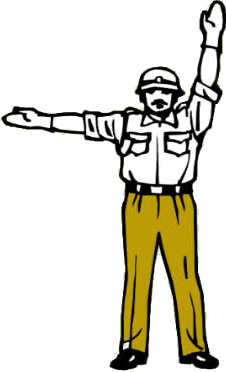
\includegraphics[height=7cm]{/content/ges-turn-right.jpg} \caption{Turn Right Gesture} \label{fg:ges:3} 
	\end{minipage}
	\begin{minipage}
		{.45 
		\textwidth} \centering 
		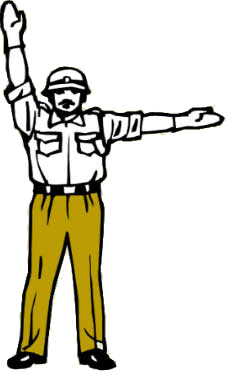
\includegraphics[height=7cm]{/content/ges-turn-left.jpg} \caption{Turn Left Gesture} \label{fg:ges:2} 
	\end{minipage}
	\begin{minipage}
		{.45 
		\textwidth} \centering 
		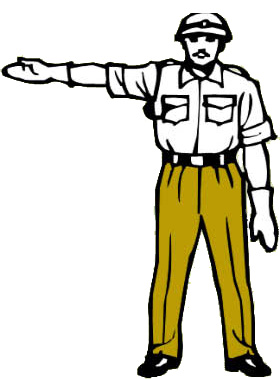
\includegraphics[height=7cm]{/content/ges-move-right.jpg} \caption{Move Right Gesture} \label{fg:ges:5} 
	\end{minipage}
	\begin{minipage}
		{.45 
			\textwidth} \centering 
		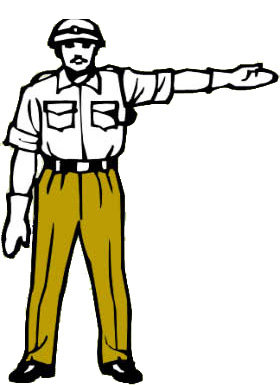
\includegraphics[height=7cm]{/content/ges-move-left.jpg} \caption{Move Left Gesture} \label{fg:ges:4} 
	\end{minipage}
	\begin{minipage}
		{.45 
		\textwidth} \centering 
		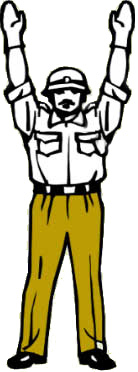
\includegraphics[height=7cm]{/content/ges-walk.jpg} \caption{Walk Gesture} \label{fg:ges:1} 
	\end{minipage}	

	\caption{In this thesis, five static hand gestures are modeled based on the traffic police hand signals. \cite{22} }
	\label{fg:ges:hands} 
\end{figure}

